% HW3 report: cover page + one page (plot + discussion). Needs plot_notes.png in the same folder.

\documentclass[11pt]{article}

\usepackage[utf8]{inputenc}
\usepackage{geometry}
\geometry{letterpaper, margin=1in}
\usepackage{setspace}
\usepackage{amsmath}
\usepackage{amssymb}
\usepackage{graphicx}
\usepackage{xcolor}
\usepackage{fancyhdr}
\usepackage{hyperref}
\hypersetup{colorlinks=true, linkcolor=blue, urlcolor=blue, pdfborder={0 0 0}}
\pagestyle{fancy}
\fancyhf{}
\fancyfoot[C]{\thepage}

\newcommand{\hwNumber}{\#3}
\newcommand{\hwTitle}{Tuning multiple notes on your instrument}

\begin{document}

%% ------------------------- Cover page -------------------------
\begin{center}
    \vspace*{2cm}
    \textbf{Vanderbilt University \\}
    \textbf{School of Engineering \\}
    \vfill
    \textbf{ES 1402-13 \\}
    \textbf{Dr. Bellan\\}
    \textbf{Fall 2026-2027\\}
    \textbf{October 28, 2026 \\}
    \textbf{HW 3: \hwTitle \\}
    \vfill
    \textbf{Youssef Nassar \\}
    (Student ID: nassary) \\
    \vfill
\end{center}

\thispagestyle{empty}
\newpage
\pagenumbering{arabic}

\fancyhead[L]{\footnotesize\textbf{Vanderbilt University}}
\fancyhead[C]{\footnotesize\textbf{\hwTitle\ \hwNumber}}
\fancyhead[R]{\footnotesize\textbf{ES 1402}}

%% ------------------------- The one page -------------------------
\setstretch{1.15}

\begin{center}
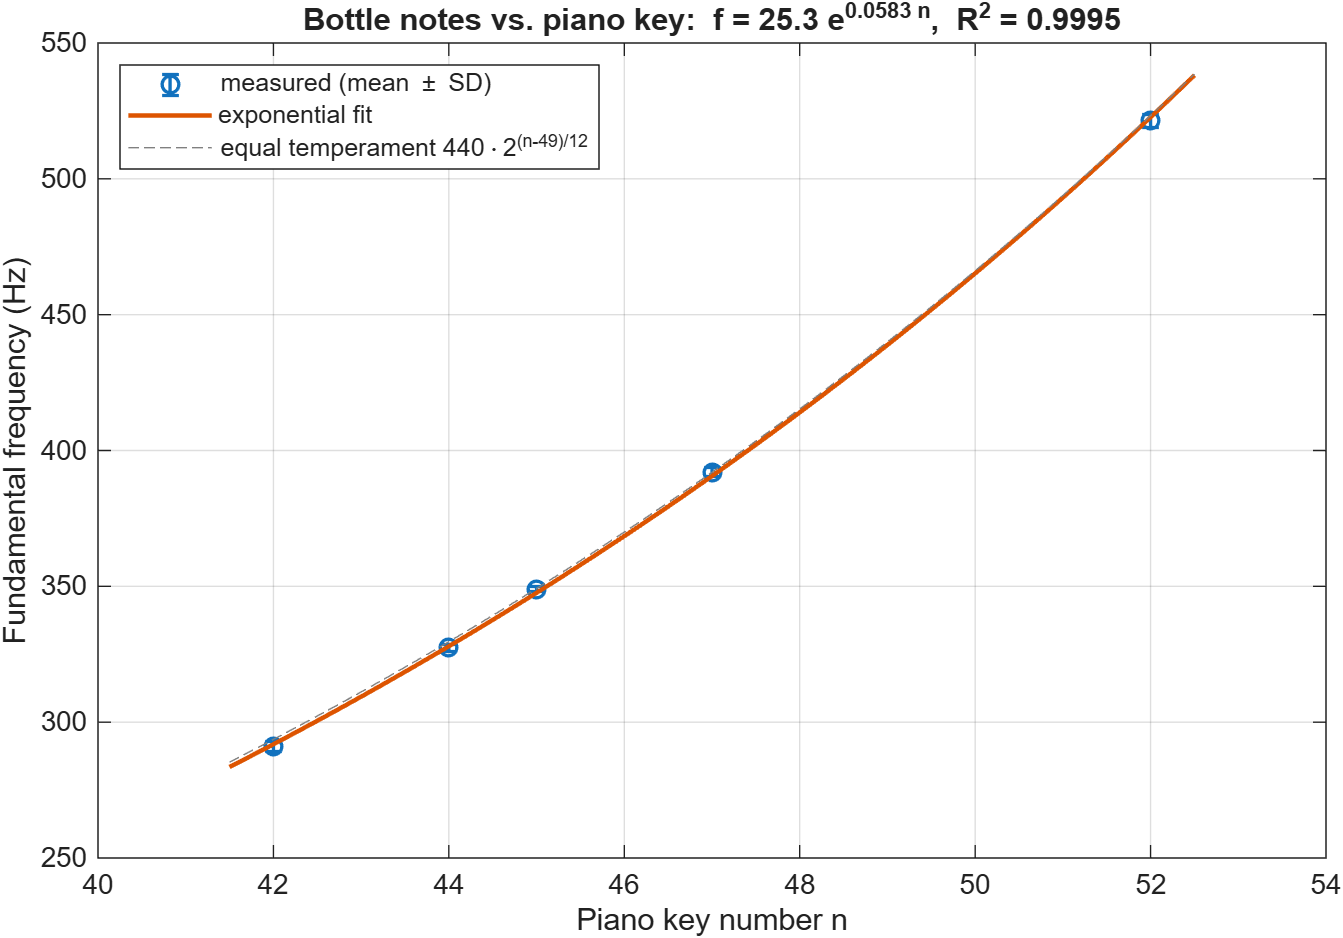
\includegraphics[width=0.9\linewidth]{plot_notes.png}\\[0.2em]
{\small\textbf{Figure 1.} Measured frequency of the five bottles vs.\ piano key number $n$ (mean $\pm$ SD of 3 readings), with the exponential fit (solid line) and the equal-temperament equation (dashed line).}
\end{center}

\vspace{0.4em}
\noindent
Five notes were made from five identical 355 mL water bottles, each one a Helmholtz resonator like the bottle from HW 2. A note is produced by blowing across the open neck of a bottle. The pitch depends on the amount of air in the bottle: more air gives a lower note, and less air gives a higher note.
All bottles were started with 343 mL of water, and the notes were tuned by taking water out, by pouring and with a syringe, until the main peak in Friture was at the wanted frequency. The notes chosen were D4 (key 42), E4 (44), F4 (45), G4 (47) and C5 (52). Lower octaves were used where possible because a bottle with more air sounded louder.
Three readings were taken for each bottle.
The piano equation, $f = 440\cdot2^{(n-49)/12}$, is exponential in the key number $n$, so an exponential fit $f = Ae^{kn}$ was used. The fit gave $f = 25.3\,e^{0.0583\,n}$ with $R^2 = 0.9995$.
The fitted values are close to the piano equation, which has $k = 0.0578$ and gives 440 Hz for key 49: the fit gave $k = 0.0583$ and 439 Hz.
The measured notes were also close to the target notes. D4 and E4 were about 1\% low (291 Hz instead of 293.7 Hz, and 327 Hz instead of 329.6 Hz), and F4, G4 and C5 were within 0.5\% of the target.
The readings of each bottle were repeatable, within about 1 to 3 Hz.
Some limitations were met. The pitch changes a lot with a small change in water, so the water level had to be adjusted carefully. The Friture peak was wide and noisy because of breath noise, so it was hard to read exactly, especially for G4. The pitch also changes a little with the way the bottle is blown.
In addition, the starting water amounts were only estimates from HW 2, so each bottle had to be tuned by trial. Finally, only five notes were measured, so a high $R^2$ does not by itself show that every note is perfectly in tune.

\end{document}
